\documentclass[11pt]{article}

\usepackage[english]{babel}
\usepackage[margin=0.8in]{geometry}

% Math/Greek packages
\usepackage{amssymb,amsmath,amsthm, mathtools} 
\usepackage{algorithm, algorithmic}
\usepackage{upgreek, siunitx}
\usepackage{setspace}

% Graphics/Presentation packages
\usepackage{multirow}
\usepackage{graphicx}
\usepackage{cancel}
\usepackage{tabulary, enumitem, array}
\usepackage{xparse,mleftright,tikz}
\usepackage{physics}

% Misc packages
\usepackage{fancyhdr}


\usepackage[export]{adjustbox}

\usepackage{esint}

\sisetup{locale=US,group-separator = {,}}
\usepackage[colorlinks=true, allcolors=blue]{hyperref}


% Box function - update this as more sophisticated solutions are found
\newcommand\mybox[2][]{\tikz[overlay]\node[fill=blue!20,inner sep=2pt, anchor=text, rectangle, rounded corners=1mm,#1] {#2};\phantom{#2}}
\renewcommand{\arraystretch}{1.2}

% General macro declarations


\makeatletter
\let\oldabs\abs
\def\abs{\@ifstar{\oldabs}{\oldabs*}}
%
\let\oldnorm\norm
\def\norm{\@ifstar{\oldnorm}{\oldnorm*}}
\makeatother

\begin{document}

\title{PHSX 462: HW04}
\author{William Jardee}
\maketitle

\section*{Griffiths 7.19}
\begin{enumerate}[label=\alph*)]
\item This is pretty straightforward, if we realize that $\vec{L}$ and $\vec{S}$ act on different basis, so they will commute. I will also do the general calculation for only one component of $L$, as the other two have an identical derivation.
\begin{align*}
\left[\vec{L}\cdot\vec{S}, \vec{L}\right] & = (\vec{L}\cdot \vec{S})\vec{L} - \vec{L}(\vec{L}\cdot\vec{S})\\
&= (L_xS_x + L_yS_y + L_zS_z)\vec{L} - \vec{L}(L_xS_x + L_yS_y + L_zS_z)\\
&= (L_xS_xL_x + L_yS_yL_x + L_zS_zL_x - L_xL_xS_x - L_xL_yS_y - L_xL_zS_z) \hat{x} + \cdots\\
&= (L^2_xS_x + L_yL_xS_y + L_zL_xS_z - L_x^2 S_x - L_xL_yS_y - L_xL_zS_z)\hat{x} + \cdots \\
&= \left[(L_yL_x - L_xL_y)S_y + (L_zL_x - L_xL_z)S_z\right]\hat{x} + \cdots\\
&= \left[-i\hbar L_zS_y + i\hbar L_yS_z\right]\hat{x} + \left[i\hbar L_xS_z - i\hbar L_zS_x\right]\hat{y} + \left[i\hbar L_xS_y - i\hbar L_y S_x\right]\hat{z}\\
&= i\hbar \vec{L}\times \vec{S}
\end{align*}
\item This is pretty much an identical calculation as part \textbf{a)}, but I have copied it for completeness.
\begin{align*}
\left[\vec{L}\cdot\vec{S}, \vec{S}\right] & = (\vec{L}\cdot \vec{S})\vec{S} - \vec{S}(\vec{L}\cdot\vec{S})\\
&= (L_xS_x + L_yS_y + L_zS_z)\vec{S} - \vec{S}(L_xS_x + L_yS_y + L_zS_z)\\
&= (L_xS_xS_x + L_yS_yS_x + L_zS_zS_x - S_xL_xS_x - S_xL_yS_y - S_xL_zS_z) \hat{x} + \cdots\\
&= (S^2_xL_x + S_yS_xL_y + S_zS_xL_z - S_x^2 L_x - S_xS_yL_y - S_xS_zL_z)\hat{x} + \cdots \\
&= \left[(S_yS_x - S_xS_y)L_y + (S_zS_x - S_xS_z)L_z\right]\hat{x} + \cdots\\
&= \left[-i\hbar S_zL_y + i\hbar S_yL_z\right]\hat{x} + \left[i\hbar S_xL_z - i\hbar S_zL_x\right]\hat{y} + \left[i\hbar S_xL_y - i\hbar S_y L_x\right]\hat{z}\\
&= i\hbar \vec{S}\times \vec{L}
\end{align*}
\item  This one is easy, let's just use the results from the previous two parts.
\begin{align*}
\left[\vec{L}\cdot \vec{S}, \vec{J}\right] & = \left[\vec{L}\cdot \vec{S}, \vec{L}+\vec{S}\right]\\
& = \left[\vec{L}\cdot \vec{S}, \vec{L}\right] + \left[\vec{L}\cdot \vec{S}, \vec{S}\right]\\
&= i\hbar \vec{L} \times \vec{S} + i\hbar \vec{S} \times \vec{L}\\
&= i\hbar \vec{L} \times \vec{S} - i\hbar \vec{L} \times \vec{S} = 0
\end{align*}
\item For this one we have to realize that $L^2$ commutes with itself, $J^2$ and $S^2$.
\begin{align*}
\left[\vec{L}\cdot \vec{S}, L^2\right] & = \frac{1}{2}\left[J^2 - L^2 - S^2, L^2\right]\\
& = \frac{1}{2}\left(\left[J^2, L^2\right] - \left[L^2, L^2\right] - \left[S^2, L^2\right]\right)\\
& = 0
\end{align*}
\item Nothing new here
\begin{align*}
\left[\vec{L}\cdot\vec{S}, S^2\right] & = \frac{1}{2}\left[J^2 - L^2 - S^2, S^2\right]\\
& = \frac{1}{2}\left(\left[J^2, S^2\right] - \left[L^2, S^2\right] - \left[S^2, S^2\right]\right)\\
&=0
\end{align*}
\item And, again!
\begin{align*}
\left[\vec{L}\cdot\vec{S}, J^2\right] & = \frac{1}{2}\left[J^2 - L^2 - S^2, J^2\right]\\
& = \frac{1}{2}\left(\left[J^2, J^2\right] - \left[L^2, J^2\right] - \left[S^2, J^2\right]\right)\\
&=0
\end{align*}

\end{enumerate}

%--------------------------------------------------------------------------------
\newpage

\section*{Griffiths 4.22 (c) and (d)}
\begin{enumerate}[label=\alph*)]
\addtocounter{enumi}{2}
\item 
These are the solutions found in the first part of the problem, and will be useful for later derivations.
\begin{align*}
\left[L_z, x\right] &= i\hbar y & \left[L_z, y\right] &= -i\hbar x & \left[L_z, z\right] & = 0\\
\left[L_z, p_x\right] &= i\hbar p_y & \left[L_z, p_y\right] &= -i\hbar p_x & \left[L_z, p_z\right] &= 0
\end{align*}
First showing that $r^2$ commutes with $L_z$:
\begin{align*}
\left[L_z, r^2\right] & = \left[L_z, x^2+y^2+z^2\right]\\
& = \left[L_z, x^2\right] + \left[L_z, y^2\right] + \left[L_z, z^2\right]\\
& =  \left[L_z, x\cdot x\right] + \left[L_z, y\cdot y\right] + \left[L_z, z\cdot z\right] \\
& = \left[L_z, x\right]x + x\left[L_z, x\right] + \left[L_z, y\right]y + y\left[L_z, y\right] + \left[L_z, z\right]z + z\left[L_z, z\right]\\
& = i\hbar yx + xi\hbar y + (-i\hbar x)y + (-i\hbar x)y +0 +0 \\
& = 0
\end{align*}
Now, showing that $p^2$ commutes with $L_z$:
\begin{align*}
\left[L_z, p^2\right] &= \left[L_z, p_x^2\right] + \left[L_z, p_y^2\right] + \left[L_z, p_z^2\right]\\
&= \left[L_z, p_x\right]p_x + p_x\left[L_z, p_x\right] + \left[L_z, p_y\right]p_y + p_y\left[L_z, p_y\right] + \left[L_z, p_z\right]p_z + p_z\left[L_z, p_z\right]\\
& = (i\hbar p_y)p_x + p_x(i\hbar p_y) + (-i\hbar p_x)p_y + p_y(-i\hbar p_x) + 0 +0 \\
&  = 0
\end{align*}
\item 
Taking a look at the Hamiltonian, remembering that in the last part we already showed that the elements of $L$ commute with $p^2$:
\begin{align*}
\left[H, L_x\right] = \left[\frac{p^2}{2m}+V, L_x\right] = \frac{1}{2m}\left[p^2, L_x\right] + \left[V, L_x\right] = 0 + \left[V(r), L_x\right]
\end{align*}
Now, we just need to show that $V(r)$ commutes with both $r$ and $r^2$. 
\begin{align*}
\left[L_x, \sqrt{x^2+y^2+z^2}\right] & = L_x\sqrt{x^2+y^2+z^2} + \sqrt{x^2+y^2+z^2}L_x \\
& = (yp_z - zp_y)\sqrt{x^2+y^2+z^2} - \sqrt{x^2+y^2+z^2}(yp_z - zp_y)\\
& = -y\frac{i\hbar}{2\sqrt{x^2+y^2+z^2}}2z + y\sqrt{x^2+y^2+z^2}p_z + z\frac{i\hbar}{2\sqrt{x^2+y^2+z^2}}2y \\
& \hspace{4em} - z\sqrt{x^2+y^2+z^2}p_y -\sqrt{x^2+y^2+z^2}(yp_z - zp_y)\\
& = y\sqrt{x^2+y^2+z^2}p_z - y\sqrt{x^2+y^2+z^2}p_z - z\sqrt{x^2+y^2+z^2}p_y \\
& \hspace{4em} + z\sqrt{x^2+y^2+z^2}p_y\\
&=0
\end{align*}
Imposing the transitive law, we can say that 
\begin{align*}
\left(\left[L^2, L_x\right]=0\right) \land \left(\left[L_x, r\right] =0 \right)\longrightarrow \left[L^2, r\right] = 0
\end{align*}
Since the eigenstates of $V(r)$ can be broken down into the eigenstates of $r$ or $r^2$, and $L^2$ and $L_x$ commute with $r$ and $r^2$, then they both commute with $V(r)$. The proof is nearly identical for $L_y$ and $L_z$. 
\end{enumerate}

%--------------------------------------------------------------------------------
\newpage

\section*{Griffiths 7.20}
\begin{equation}
E^1_{fs} = \frac{\left(E_n\right)^2}{2mc^2}\left(3 - \frac{4n}{j+1/2}\right)
\tag{Equation 7.68}
\end{equation}
\begin{equation}
E_r^1 = -\frac{(E_n)^2}{2mc^2}\left(\frac{4n}{l+1/2} - 3\right)
\tag{Equation 7.58}
\end{equation}
\begin{equation}
E^1_{so} = \frac{(E_n)^2}{mc^2}\left[\frac{n(j(j+1)-l(l+1)-3/4)}{l(l+1/2)(l+1)}\right]
\tag{Equation 7.67}
\end{equation}
We are trying to derive Equation 7.68 from Equation 7.58 and Equation 7.67. Let us do the case where $j=l+1/2$ first:
\begin{align*}
E_{fs}^1 &= E_r^1 + E_{so}^1\\
&= -\frac{(E_n)^2}{mc^2}\left[\frac{4n}{l+\frac{1}{2}} -3\right] + \frac{(E_n)^2}{mc^2}\left[\frac{n\left[j(j+1)-l(l+1)-\frac{3}{4}\right]}{l(l+1/2)(l+1)}\right]\\
&= \frac{(E_n)^2}{2mc^2}\left[\frac{-4n(l)(l+1)+2n(j(j+1)-l(l+1)-3/4)}{l(l+1/2)(l+1))}+3\right]
\end{align*}
Looking at just the numerator:
\begin{align*}
&-4n\left(j+\frac{1}{2}\right)\left(j+\frac{3}{2}\right)+2n\left[j(j+1) -\left(j+\frac{1}{2}\right)\left(j+\frac{3}{2}\right)-\frac{3}{4}\right]\\
&\quad = -n\left[4j^2 + 10j+6\right]\\
&\quad = -2n(2j+3)(j+1)\\
&\quad = -4n\left(j+\frac{3}{2}\right)\left(j+1\right)
\end{align*}
At the same time, the numerator becomes:
\[\left(j+\frac{1}{2}\right)(j+1)\left(j+\frac{3}{2}\right)\]
\begin{align*}
E_{fs}^1 & =\frac{(E_n)^2}{2mc^2}\left[\frac{-4n\left(j+\frac{3}{2}\right)(j+1)}{\left(j+\frac{1}{2}\right)(j+1)\left(j+\frac{3}{2}\right)}+3\right]\\
& = \frac{(E_n)^2}{2mc^2}\left[3-\frac{4n}{j+\frac{1}{2}}\right] \quad \checkmark
\end{align*}

Doing this same math for $j-1/2$; jumping straight to the part were we analyze the numerator and plugged in $j$ for $l$:
\begin{align*}
&-4n\left(j-\frac{1}{2}\right)\left( j +\frac{1}{2}\right) + 2n\left[j(j+1)-\left(j-\frac{1}{2}\right)\left(j+\frac{1}{2}\right)-\frac{3}{4}\right]\\
& \quad = -4n\left(j^2-\frac{1}{4}\right) + 2n\left[j^2 +j-j^2+\frac{1}{4}-\frac{3}{4}\right]\\
& \quad = n\left[-4j^2+2j\right]\\
& \quad = -4nj\left(j-\frac{1}{2}\right)
\end{align*}
The denominator becomes:
\[\left(j-\frac{1}{2}\right)j\left(j+\frac{1}{2}\right)\]
So:
\begin{align*}
E_{fs}^1 & = \frac{(E_n)^2}{2mc^2}\left[\frac{-4nj\left(j-\frac{1}{2}\right)}{\left(j-\frac{1}{2}\right)j\left(j+\frac{1}{2}\right)}+3\right]\\
& = \frac{(E_n)^2}{2mc^2}\left[3-\frac{4n}{j+\frac{1}{2}}\right] \quad \checkmark
\end{align*}

%--------------------------------------------------------------------------------
\newpage

\section*{Griffiths 7.21}

First, we need to get the general jumps: 
\begin{align*}
E_2 & = -\frac{13.6 \text{eV}}{4} & E_3 & = -\frac{13.6 \text{eV}}{9}
\end{align*}

Next, we can use Equation 7.68 (from the previous problem) to calculate each of the correction energies:
\begin{align*}
E^1_{fs}(n=2, j=1/2) & = -\frac{(13.6 \text{eV})^2}{2(4)^2 m_ec^2}\cdot 5 & E^1_{fs}(n=2, j=3/2) &= -\frac{(13.6 \text{eV})^2}{2(4)^2 m_ec^2}\\
E^1_{fs}(n=3, j=1/2) & = -\frac{(13.6 \text{eV})^2}{2(9)^2m_ec^2}\cdot 9 & E^1_{fs}(n=3, j=3/2)& = - \frac{(13.6 \text{eV})^2}{2(9)^2m_ec^2}\cdot 3 \\
E^1_{fs}(n=3, j=5/2) & = -\frac{(13.6 \text{eV})^2}{2(9)^2m_ec^2}
\end{align*}

The $n=2$ level splits into two different energy levels, and the $n=3$ splits into three different energy levels.

Finally, passing these values to a Python script:
\begin{table}[!ht]
\centering
\begin{tabular}{r | c c}
Transition & $\Delta$Energy & Photon $\lambda$ \\\hline
$E_3(j=1/2) \rightarrow E_2(j=3/2)$ & $1.888753$eV & $656.434$nm\\
$E_3(j=3/2) \rightarrow E_2(j=3/2)$ & $1.888874$eV & $656.392$nm\\
$E_3(j=5/2) \rightarrow E_2(j=3/2)$ & $1.888914$eV & $656.378$nm\\
$E_3(j=1/2) \rightarrow E_2(j=1/2)$ & $1.888934$eV & $656.371$nm\\
$E_3(j=3/2) \rightarrow E_2(j=3/2)$ & $1.889055$eV & $656.329$nm\\
$E_3(j=5/2) \rightarrow E_2(j=3/2)$ & $1.889095$eV & $656.315$nm\\
\end{tabular}
\end{table}
 	
The distance between the lines, going down the list: 
\[\boxed{0.042 \text{nm, }0.014 \text{nm, }0.007 \text{nm, }0.042\text{nm, }0.014 \text{nm}}\]

%--------------------------------------------------------------------------------
\newpage

\section*{Griffiths 7.24}
\begin{figure}[!ht]
\centering
	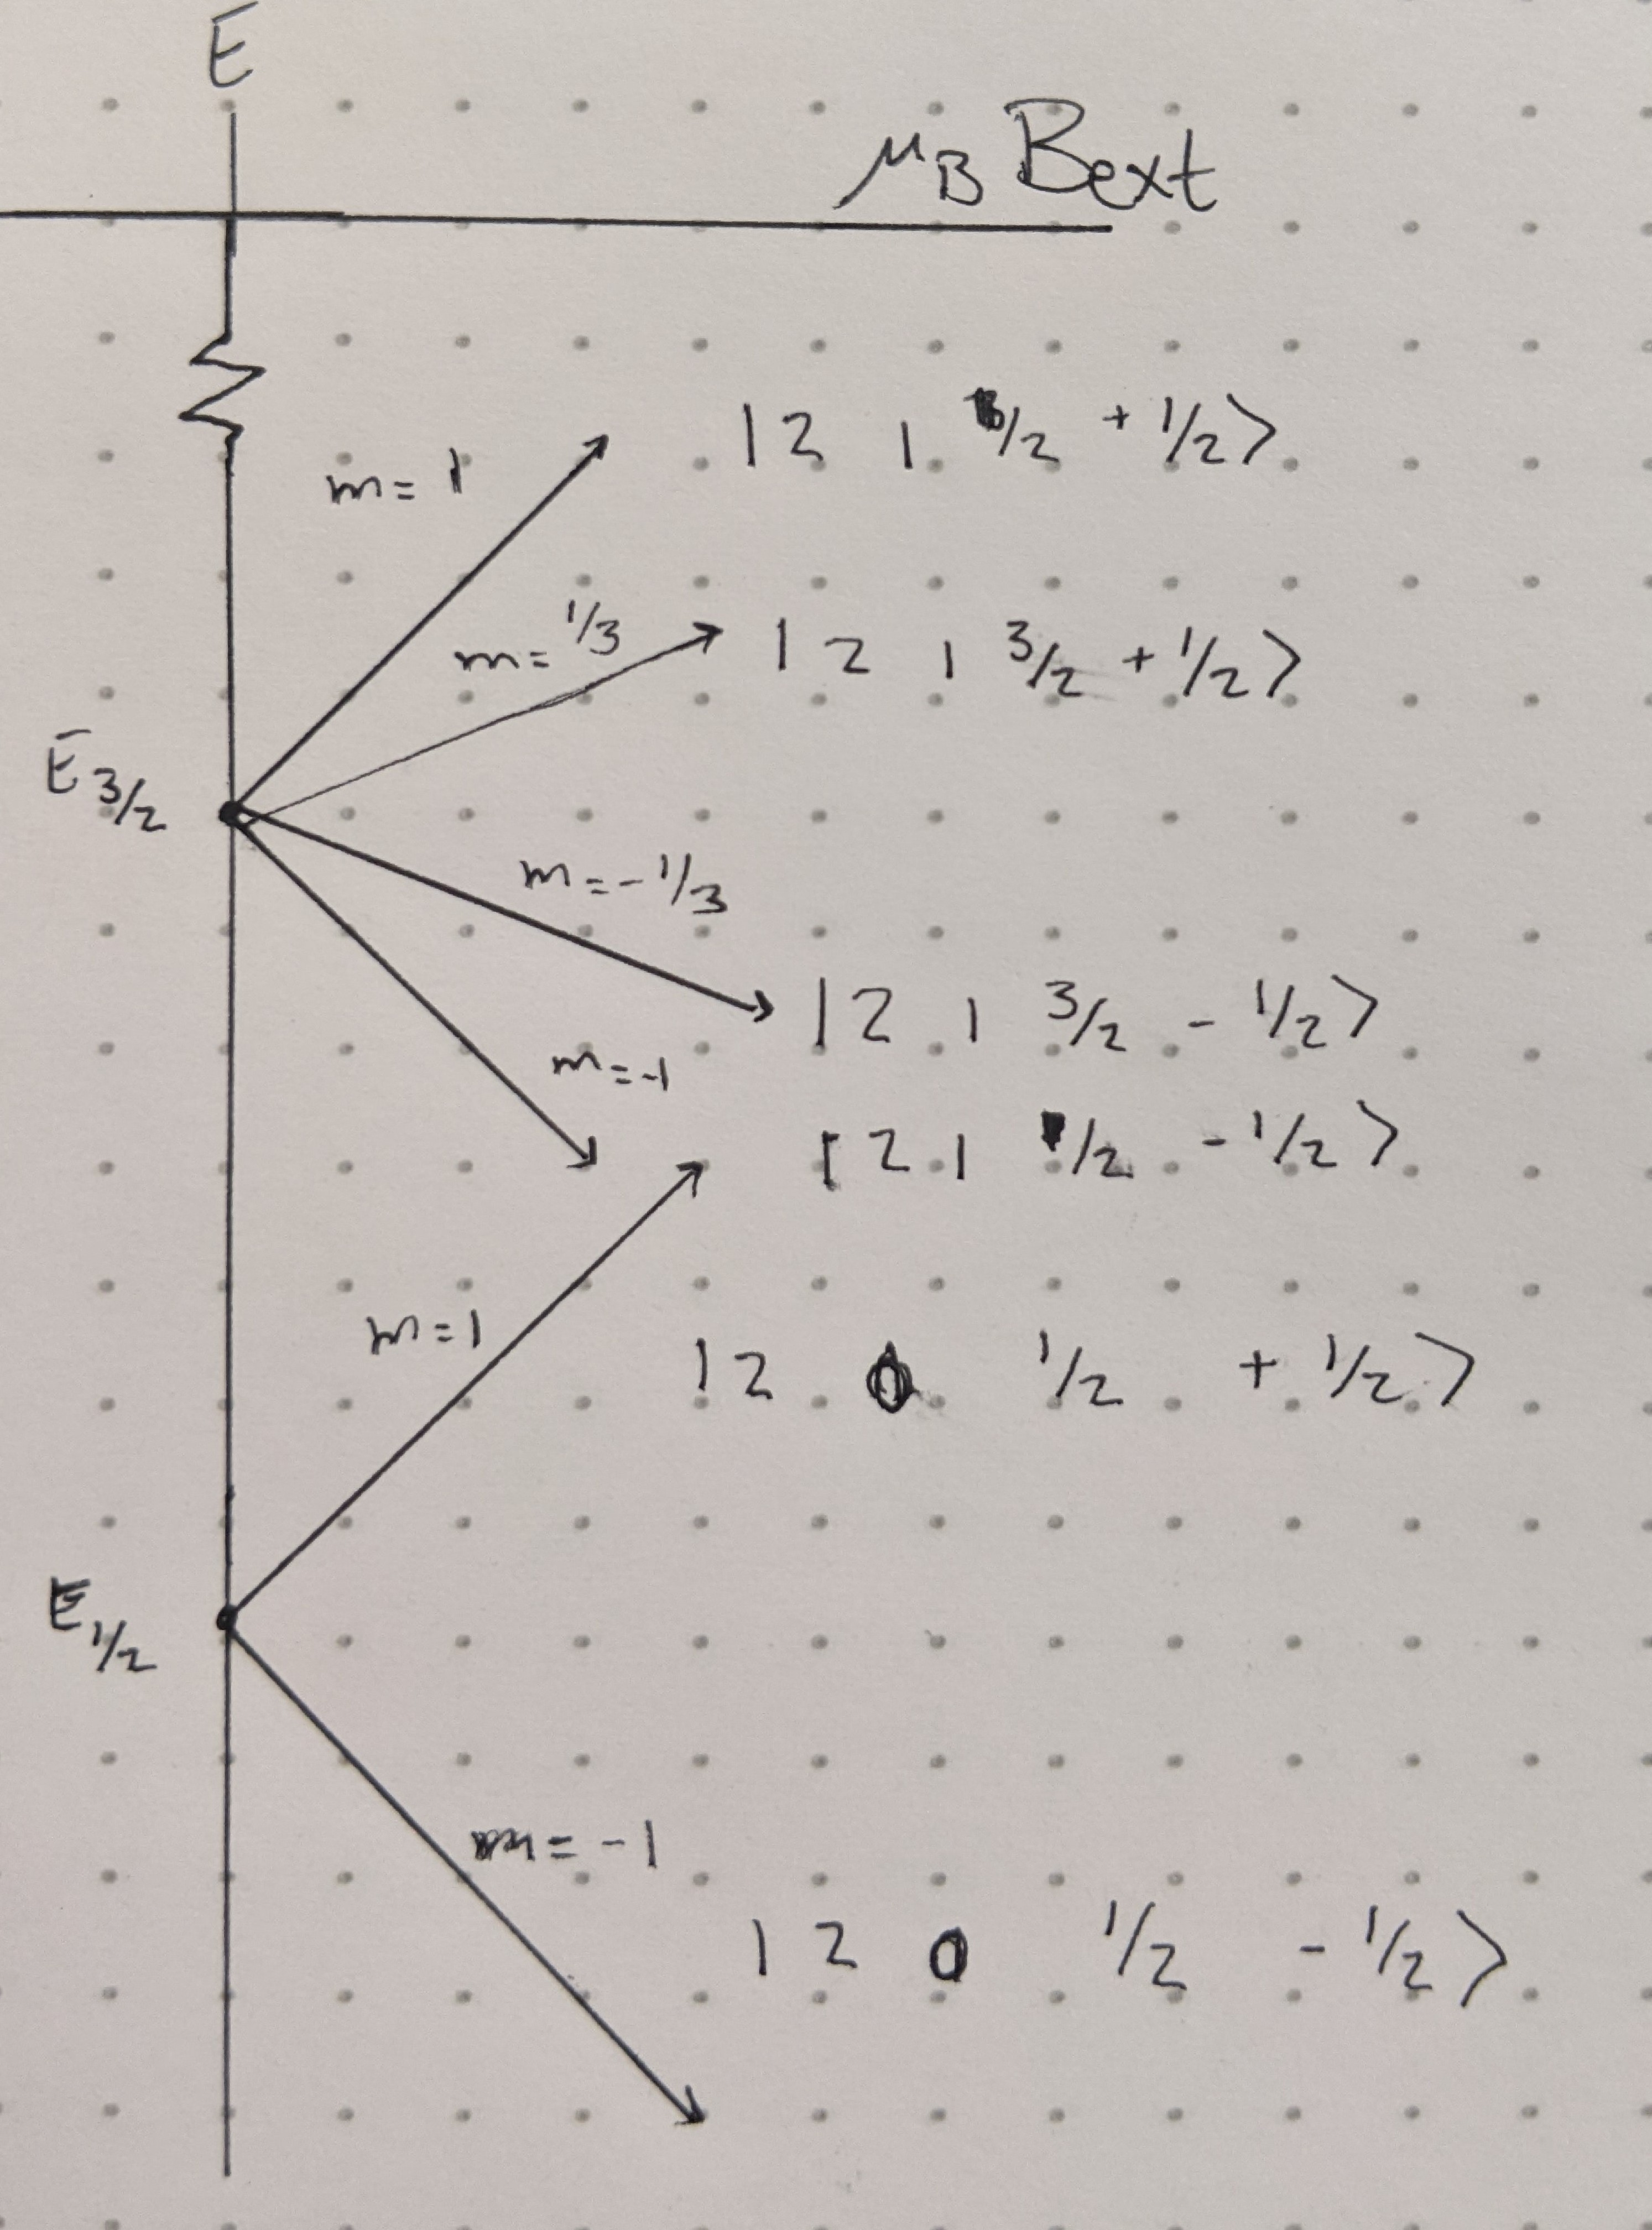
\includegraphics[scale=0.075]{phsx462_hw04_01.jpg}
	\caption{The energy levels, as a function of $\mu_B B_\text{ext}$.}
	\label{fig:5.1}
\end{figure}

Following the derivation used in the book, first we need to find the unperturbed energy (Bohr energy), then we need to find both the fine-structure correction, then the Zeeman correction. Aligning the $\vec{B}_\text{ext}$ along the $\hat{z}$ direction:
\[E^0 = -\frac{13.6 \text{eV}}{4}\]
\[E_{fs}^1 = \frac{(E_n)^2}{2m_ec^2}\left[3 - \frac{4n}{j+\frac{1}{2}}\right] \rightarrow \frac{(13.6\text{eV})^2}{2(4)^2m_ec^2}\left[3-\frac{8}{j+\frac{1}{2}}\right]\]
\[E_z^1 = \frac{e\hbar}{2m}g_jB_\text{ext}m_j\]
Where $m_e \approx 0.511$MeV$/c^2$, and $g_j = \displaystyle{\left[1 + \frac{j(j+1)-l(l+1) + s(s+1)}{2j(j+1)}\right]\ev{\vec{J}}}$. So, $g_{1/2} = 2$ and $g_{3/2} = \frac{2}{3}$

Putting this all together, we get the following energies:
\[\boxed{E = \left\{\mqty{E^0 + E^1_{fs(1/2)} \pm \mu_B B_\text{ext} & \quad \text{for } \ket{2\,1\,\frac{1}{2}\,\pm\frac{1}{2}} \\ E^0 + E^1_{fs(3/2)} \pm \mu_B \left(\frac{1}{3}\right)B_\text{ext} & \quad \text{for } \ket{2\,1\,\frac{3}{2}\,\pm\frac{1}{2}} \\ E^0 + E^1_{fs(3/2)} \pm \mu_B B_\text{ext} & \quad \text{for } \ket{2\,1\,\frac{3}{2}\,\pm\frac{3}{2}}}\right.}\]

For the graph I have labeled the two energies that get augmented as:
\begin{align*}
E_{1/2} & = E^0 + E^1_{fs(1/2)} =  -\frac{13.6 \text{eV}}{4}\left( 1 + 5\frac{13.6 \text{eV}}{8m_ec^2}\right),  & E_{3/2} &= E^0 + E^1_{fs(3/2)} = -\frac{13.6 \text{eV}}{4}\left( 1 + \frac{13.6 \text{eV}}{8m_ec^2}\right)
\end{align*}
The plotting of these energies can then be seen in Figure~\ref{fig:5.1}.

\end{document}
